\chapter{Performance Testing and user perception}
\label{cha:performance}

\section{Testing setup}

\subsection{Testing devices}

\begin{table}
  \centering
  \begin{threeparttable}
    \caption{The table shows a list of low-end testing devices.}
    \label{tab:lowendTestingDevices}
    \centering
    \def\rr{\rightskip=0pt plus1em \spaceskip=.3333em \xspaceskip=.5em\relax}
    \setlength{\tabcolsep}{1ex}
    \def\arraystretch{1.20}
    \setlength{\tabcolsep}{1ex}
    \small
    \begin{english}
      \begin{tabular}{|c||c|c|c|}
        \hline
          \multicolumn{1}{|c||}{\emph{Device}}&
          \multicolumn{1}{|c}{\emph{CPU}} &
          \multicolumn{1}{|c}{\emph{GPU}} &
          \multicolumn{1}{|c|}{\emph{RAM}} \\
        \hline
        \hline
        OnePlus 1 & 
        Snapdragon 801 & 
        Adreno 330 & 
        3GB \\
        \hline
        OnePlus 5T & 
        Snapdragon 835 & 
        Adreno 540  & 
        8GB \\
        \hline
        Samsung G\tnote{1} \hspace{0.1mm} S8 & 
        Exynos 8895 & 
        Mali-G71 MP20 & 
        4GB \\
        \hline
        Samsung GT\tnote{2} \hspace{0.1mm} A10.1 &
        Exynos 7870 & 
        Mali-T830 MP2 & 
        3GB \\
        \hline
        SurfaceBook & 
        Intel i5-6300U & 
        Intel HD 520 & 
        8GB \\
        \hline
      \end{tabular}  
    \end{english}
    \begin{tablenotes}
    \item [1] Galaxy
    \item [2] Galaxy Tab
    \end{tablenotes}
  \end{threeparttable}
\end{table}

The amount of test devices should be as high as possible while still being reasonable regarding to the effort it takes to process all resulting benchmark data. A total amount of 10 devices is enough to retrieve scientifically significant results. The range of devices is divided into 2 sections: high-end devices and low-end devices. 

The mobile devices used for testing are a OnePlus 1 phone, a OnePlus 5t phone, a Samsung Galaxy S8 phone, a SurfaceBook in tablet mode and a Samsung Galaxy Tab. All low-end devices and their specs are listed in table \ref{tab:lowendTestingDevices}. It must be noted, that every selected low-end device has a monitor refresh rate of 60-hertz. 

The table \ref{tab:highendTestingDevices} shows all high-end devices which have a monitor refresh rate of 144-hertz. It must be noted, that there are several custom tower builds with custom specs and one laptop with specs defined by its manufacturer. All in all the devices should provide a good overview of the performance of the force graph components.

\begin{table}
  \centering
  \begin{threeparttable}
    \caption{The table shows a list of high-end high refresh rate testing devices.}
    \label{tab:highendTestingDevices}
    \centering
    \def\rr{\rightskip=0pt plus1em \spaceskip=.3333em \xspaceskip=.5em\relax}
    \setlength{\tabcolsep}{1ex}
    \def\arraystretch{1.20}
    \setlength{\tabcolsep}{1ex}
    \small
    \begin{english}
      \begin{tabular}{|c||c|c|c|c|}
        \hline
          \multicolumn{1}{|c||}{\emph{Device}}&
          \multicolumn{1}{|c}{\emph{CPU}} &
          \multicolumn{1}{|c}{\emph{GPU}} &
          \multicolumn{1}{|c|}{\emph{RAM}} \\
        \hline
        \hline
        Tower (Max Z.) & 
        Intel i9-7900X & 
        2x Nvidia GTX 1080Ti & 
        32GB \\
        \hline
        Razer Blade 15 (2018) & 
        Intel i7-8750H & 
        Nvidia GTX 1070 Max-Q  & 
        16GB \\
        \hline
        Tower (Max J.) & 
        Intel i7-7700k & 
        Nvidia GTX 1070 & 
        16GB \\
        \hline
        Tower (Patrick M.) &
        Intel i7-6700k & 
        Nvidia GTX 1080 & 
        3GB \\
        \hline
        Tower (Julian J.) & 
        Intel i7-7700k & 
        Nvidia GTX 1070 & 
        16GB \\
        \hline
      \end{tabular}  
    \end{english}
  \end{threeparttable}
\end{table}

\subsection{Testing methodologies}

Running the benchmarks to get valid and scientific testing results is relatively straight forward. To get the most declarative performance numbers it is best to mainly use devices with a high monitor refresh rate. Devices with a low monitor refresh rate can possibly falsify some testing results. If for example a browser could possibly render 100 frames per second on an iteration, a system with a 60-hertz monitor would only be able to measure a maximum of 60FPS as the theoretically possible 100 FPS would be capped to the monitor's 60-hertz refresh rate.

Devices with high refresh rates can be sufficient for measuring the best performing prototype. One of the more interesting research aspects of the thesis though is the question, how well the prototypes perform on mobile devices with lower performance specifications than desktop PCs. Thus the testing results must be split up into different categories as a consequence. Due to the fact that not only frames per second, but also other perfromance aspects like total execution time are measured, the lower performing devices can also be compared to each other. All test results can also be normalized by showing a percentage of how much the performance changed across all iterations.

Each device runs through 6 iterations with exponentially increasing render difficulty. Each iteration runs through 10 cycles which equals a grand total of 60 cycles per browser and device combination. Five high-end devices with 144-hertz monitors and the five low-end devices with 60-hertz monitors run the benchmark iterations in the Chrome and in the Firefox browser. The two browsers were selected, because they're the most significantly used brwosers worldwide according to various statistics. 

\section{Benchmark Results}

\subsection{Introducing the test results}

\begin{figure}
\centering
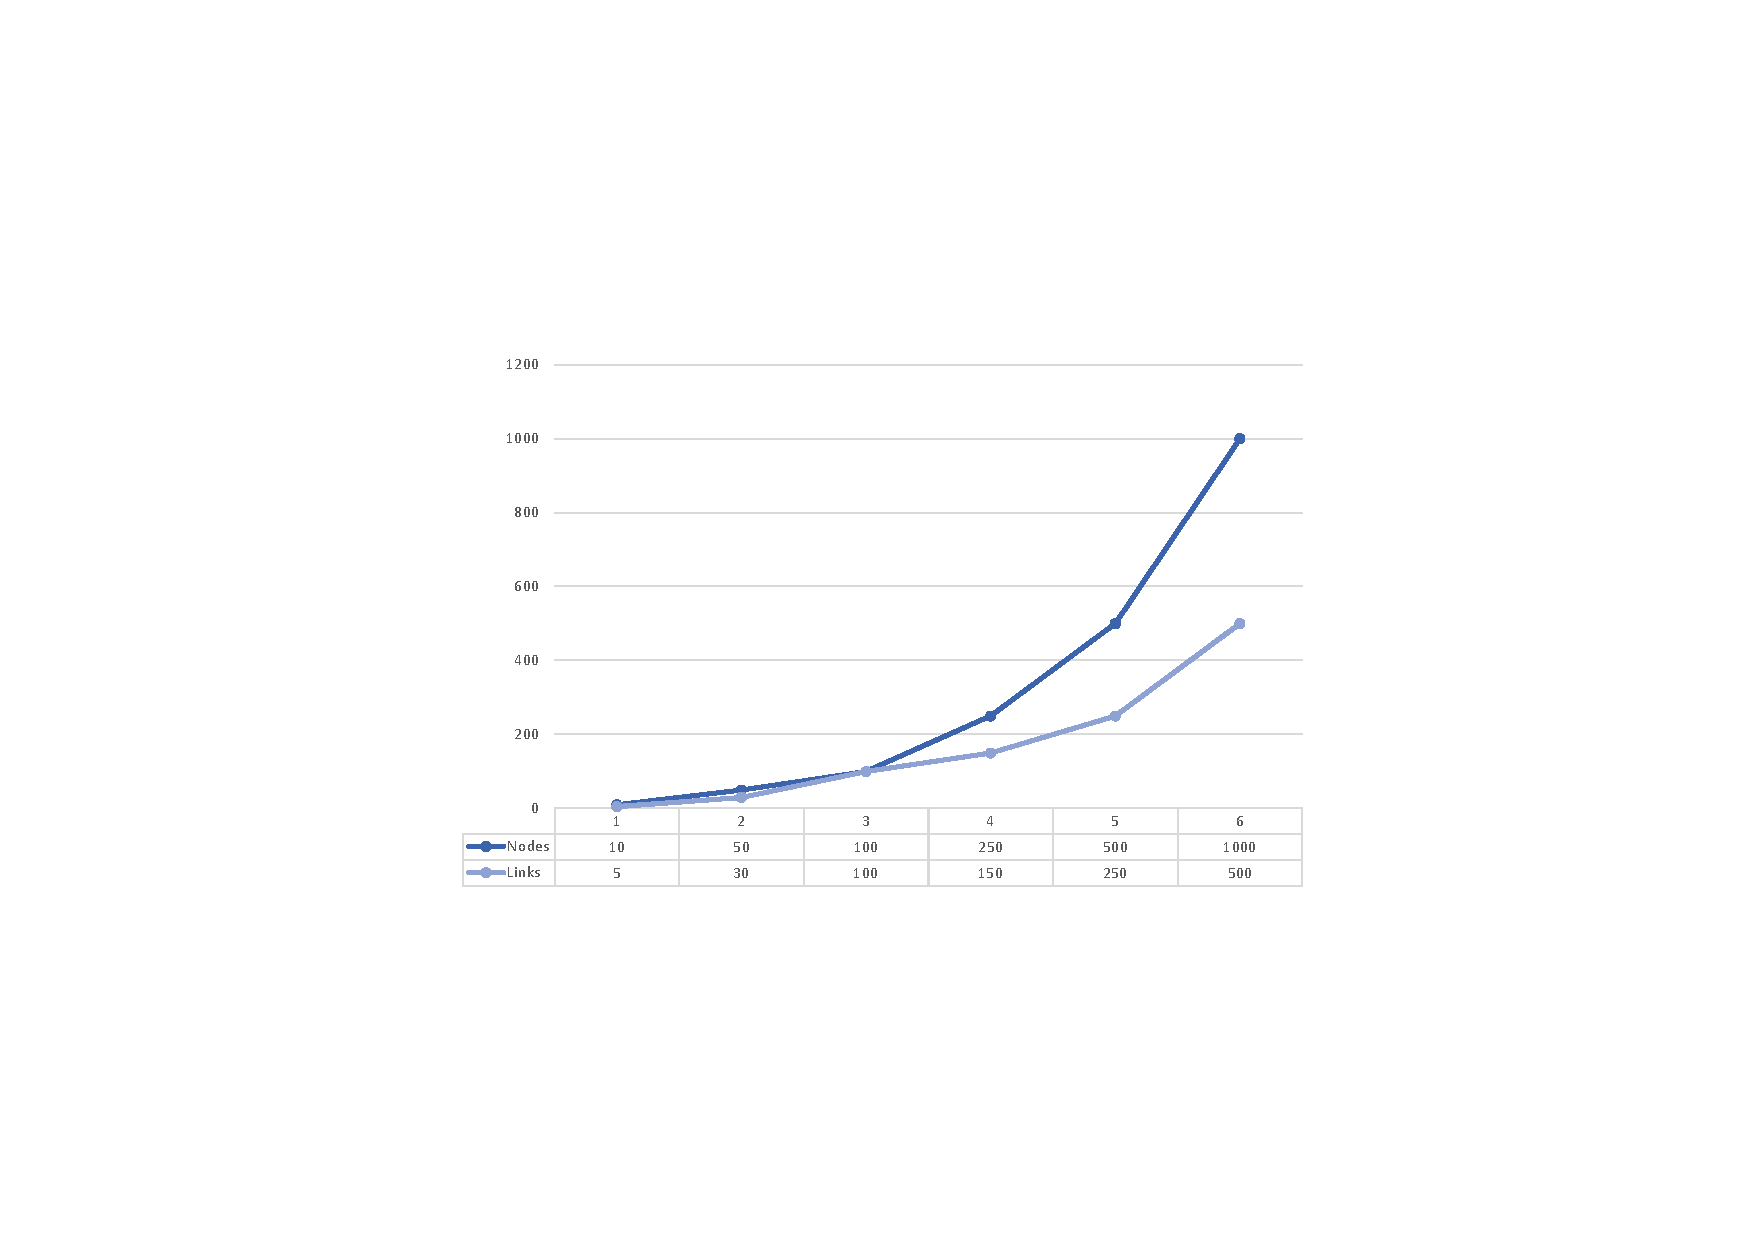
\includegraphics[scale=2.5, trim= 4cm 5cm 4cm 5cm, clip, width=1\columnwidth]{perfIterations.pdf}
\caption{Benchmark iteration configuration}
\label{fig:perfIterations}
\end{figure}

\begin{figure}
\centering
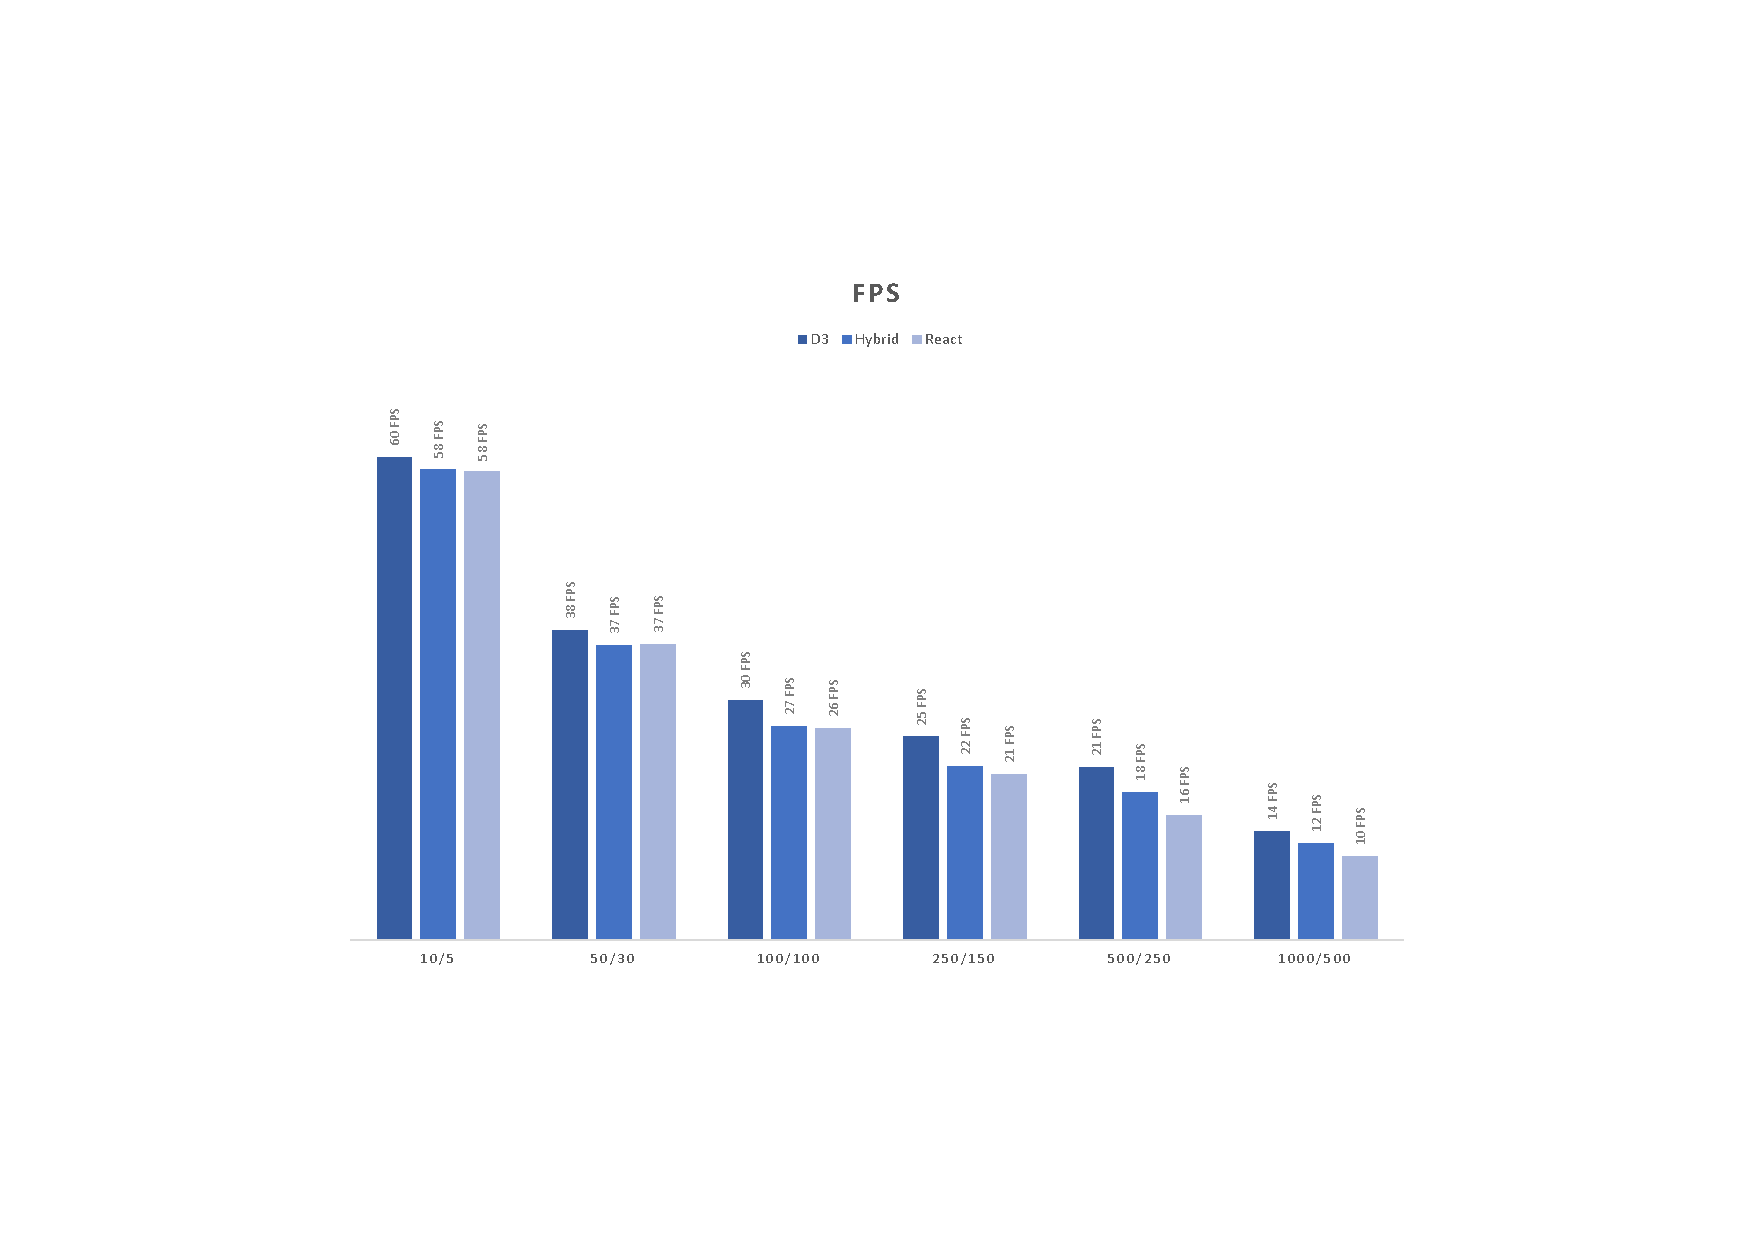
\includegraphics[scale=2.5, trim= 4cm 4cm 4cm 4cm, clip, width=1\columnwidth]{perfLowEnd001.pdf}
\caption{Average frames per second per benchmark iteration cycle}
\label{fig:perfLowEnd001}
\end{figure}

\begin{figure}
\centering
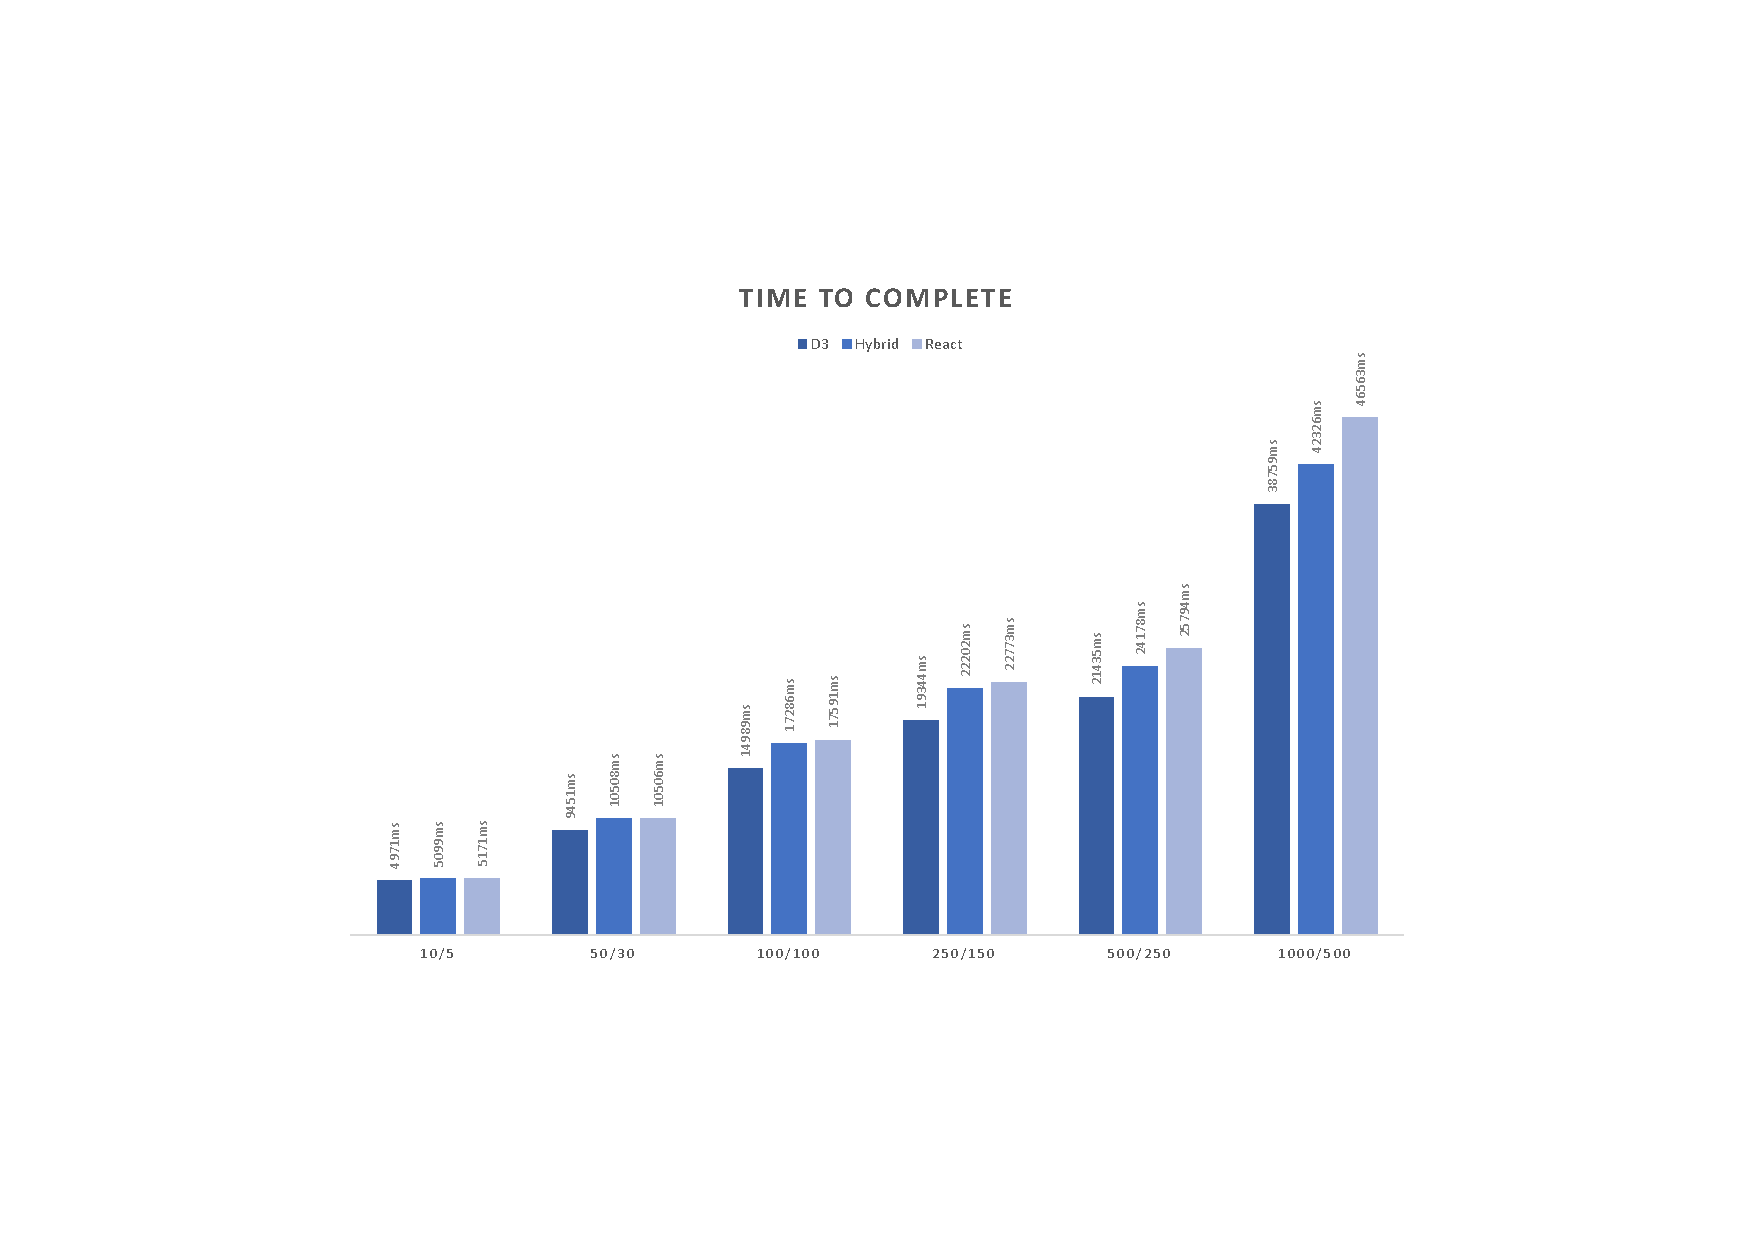
\includegraphics[scale=2.5, trim= 4cm 4cm 4cm 4cm, clip, width=1\columnwidth]{perfLowEnd002.pdf}
\caption{Average time to complete for one benchmark iteration cycle in milliseconds}
\label{fig:perfLowEnd002}
\end{figure}

\begin{figure}
\centering
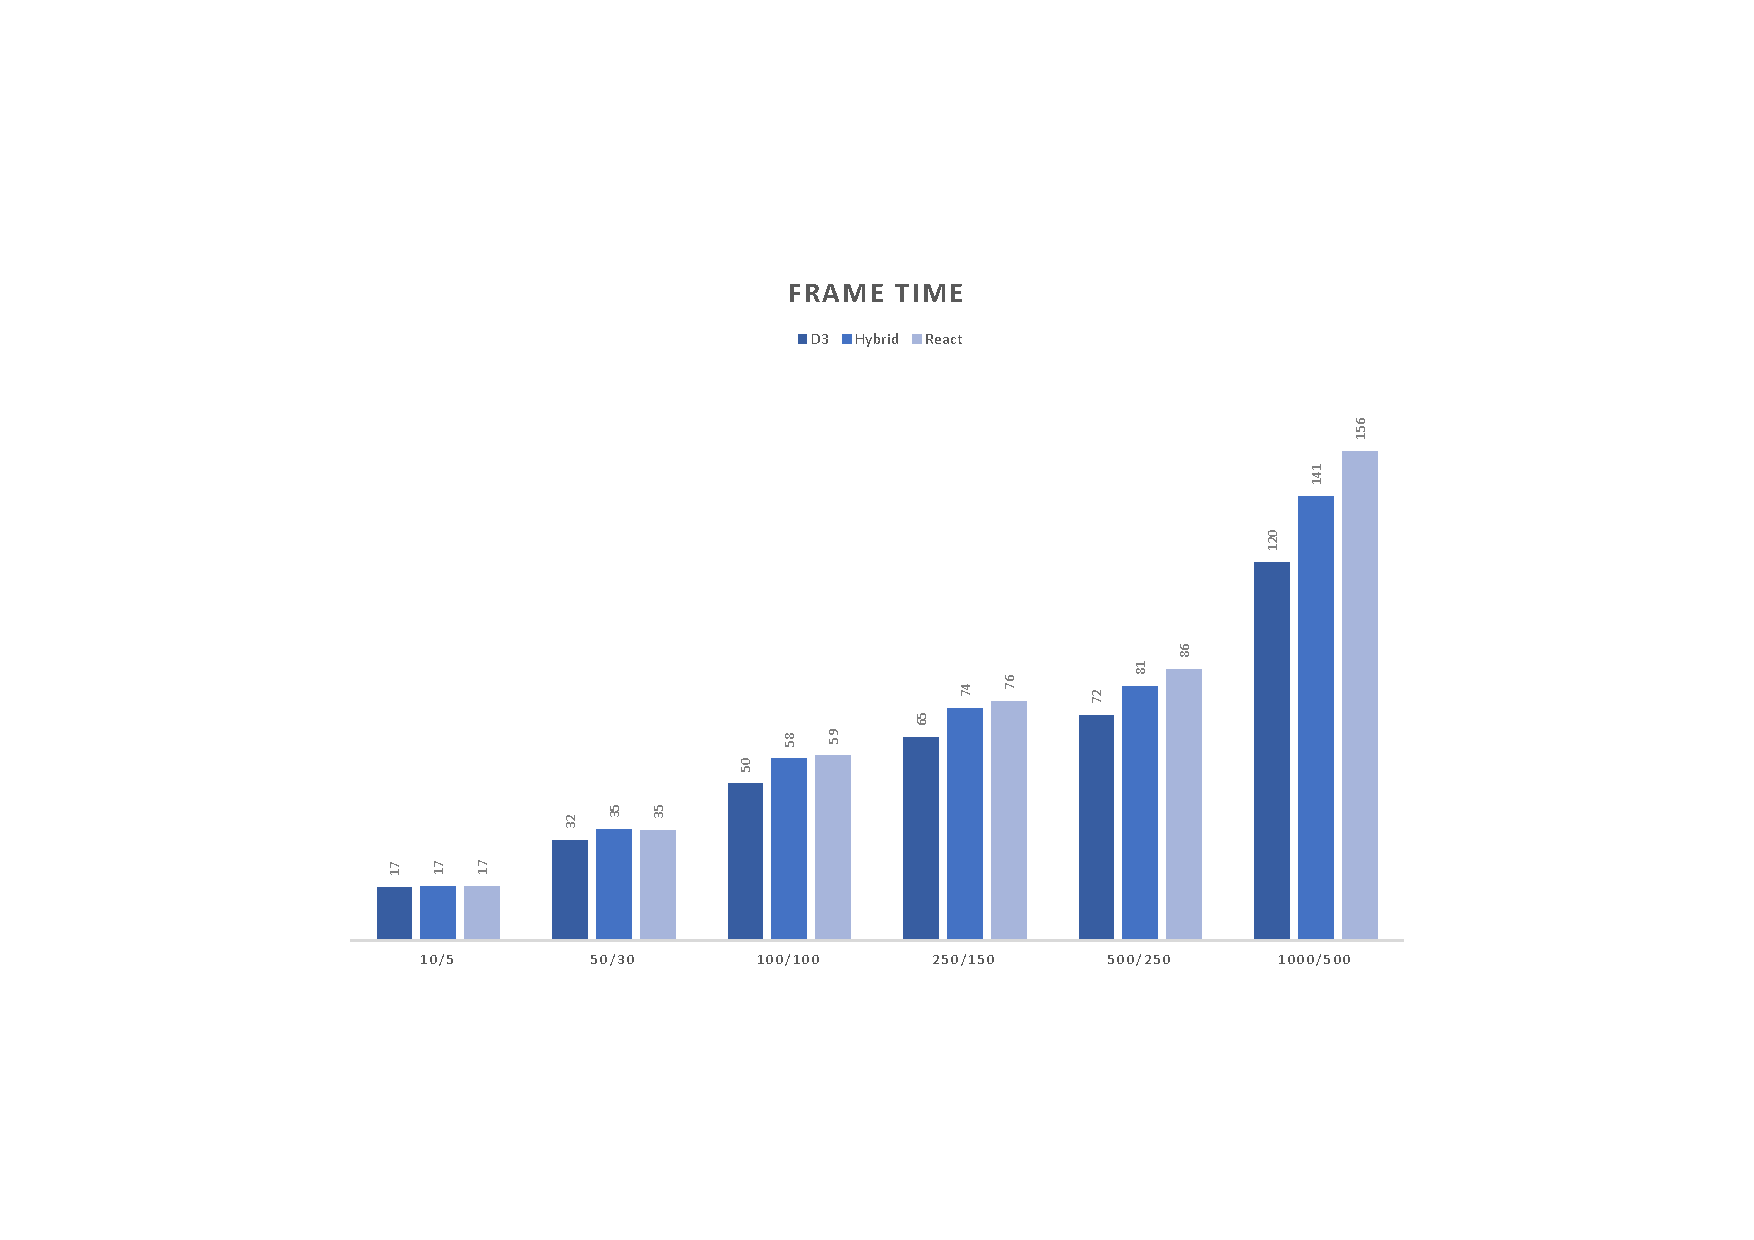
\includegraphics[scale=2.5, trim= 4cm 4cm 4cm 4cm, clip, width=1\columnwidth]{perfLowEnd003.pdf}
\caption{Average frametime per benchmark iteration cycle}
\label{fig:perfLowEnd003}
\end{figure}

\begin{figure}
\centering
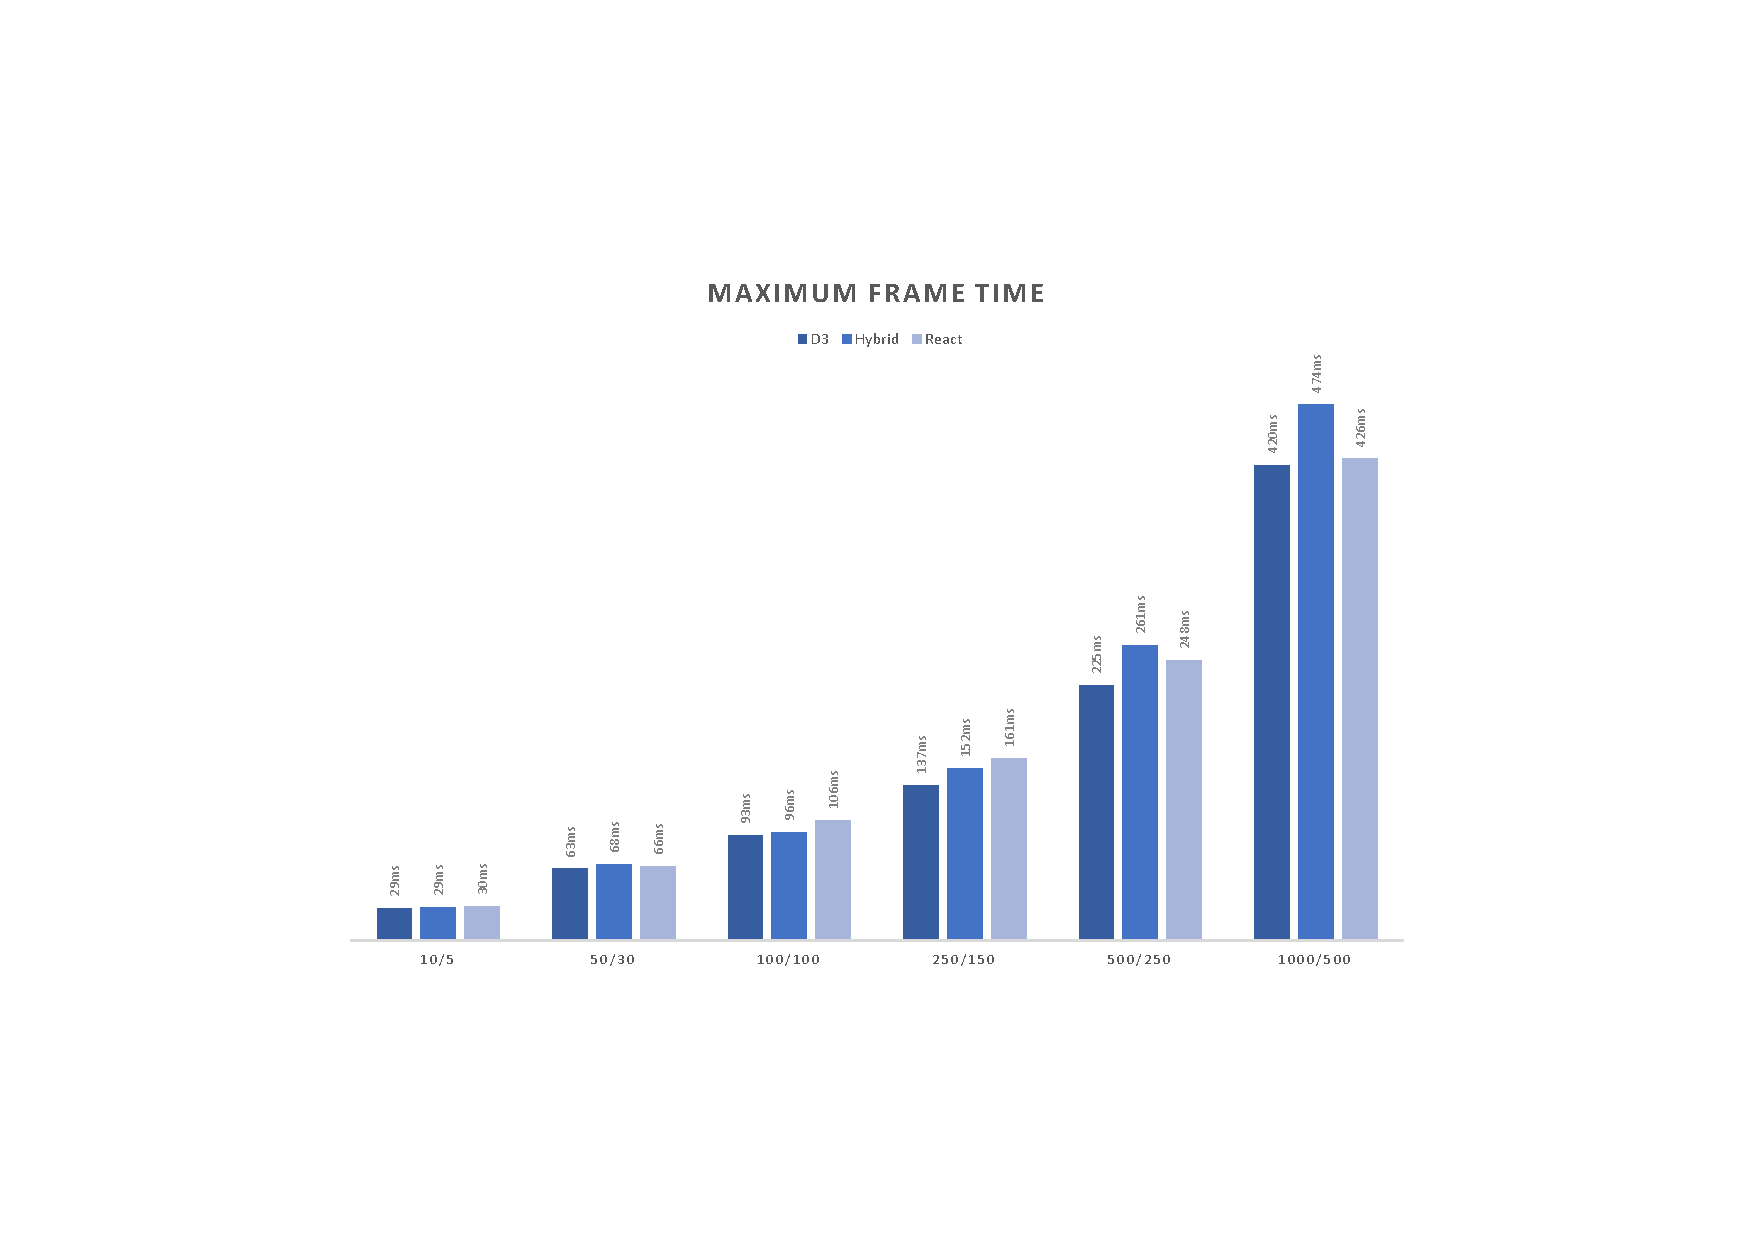
\includegraphics[scale=2.5, trim= 4cm 4cm 4cm 4cm, clip, width=1\columnwidth]{perfLowEnd004.pdf}
\caption{Average maximum frametime per benchmark iteration cycle}
\label{fig:perfLowEnd004}
\end{figure}

\begin{figure}
\centering
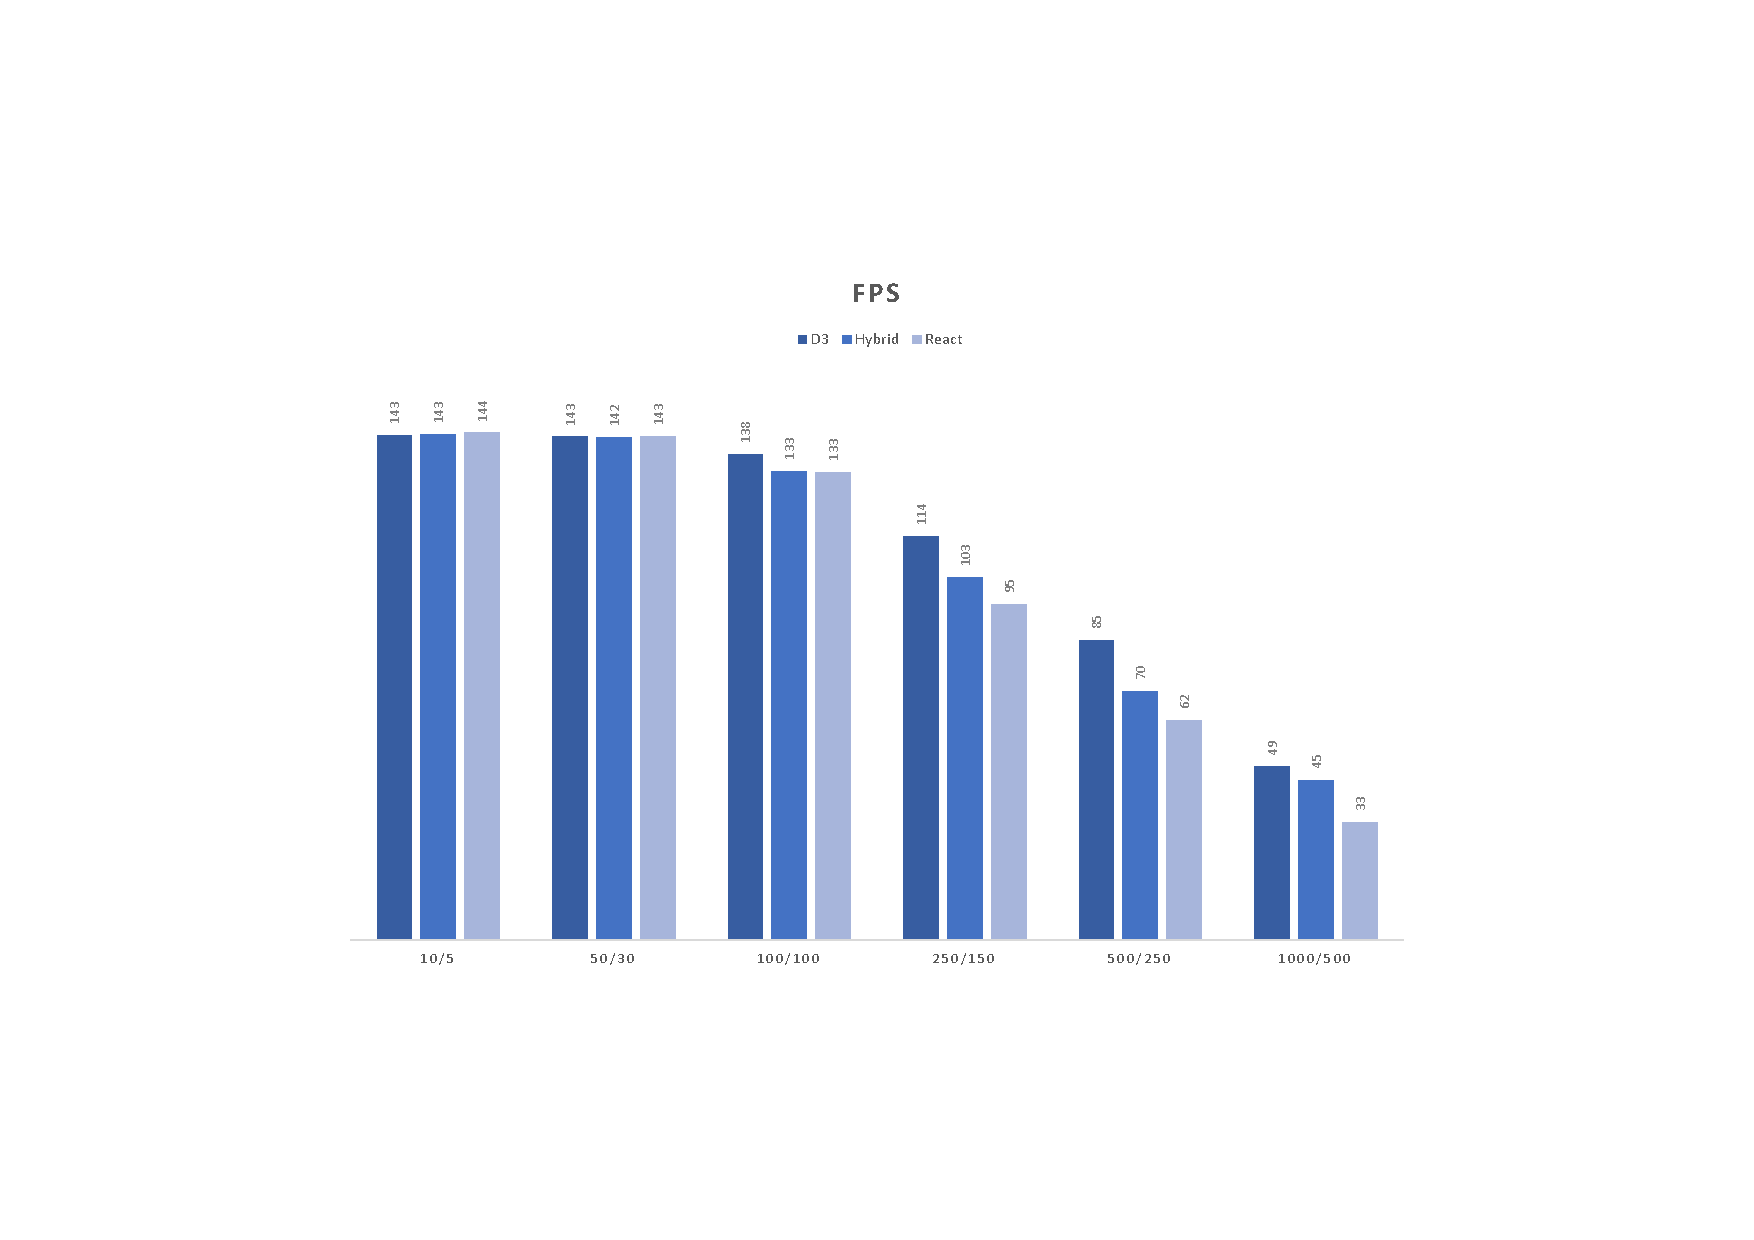
\includegraphics[scale=2.5, trim= 4cm 4cm 4cm 4cm, clip, width=1\columnwidth]{perfHighEnd001.pdf}
\caption{Average frames per second per benchmark iteration cycle}
\label{fig:perfHighEnd001}
\end{figure}

\begin{figure}
\centering
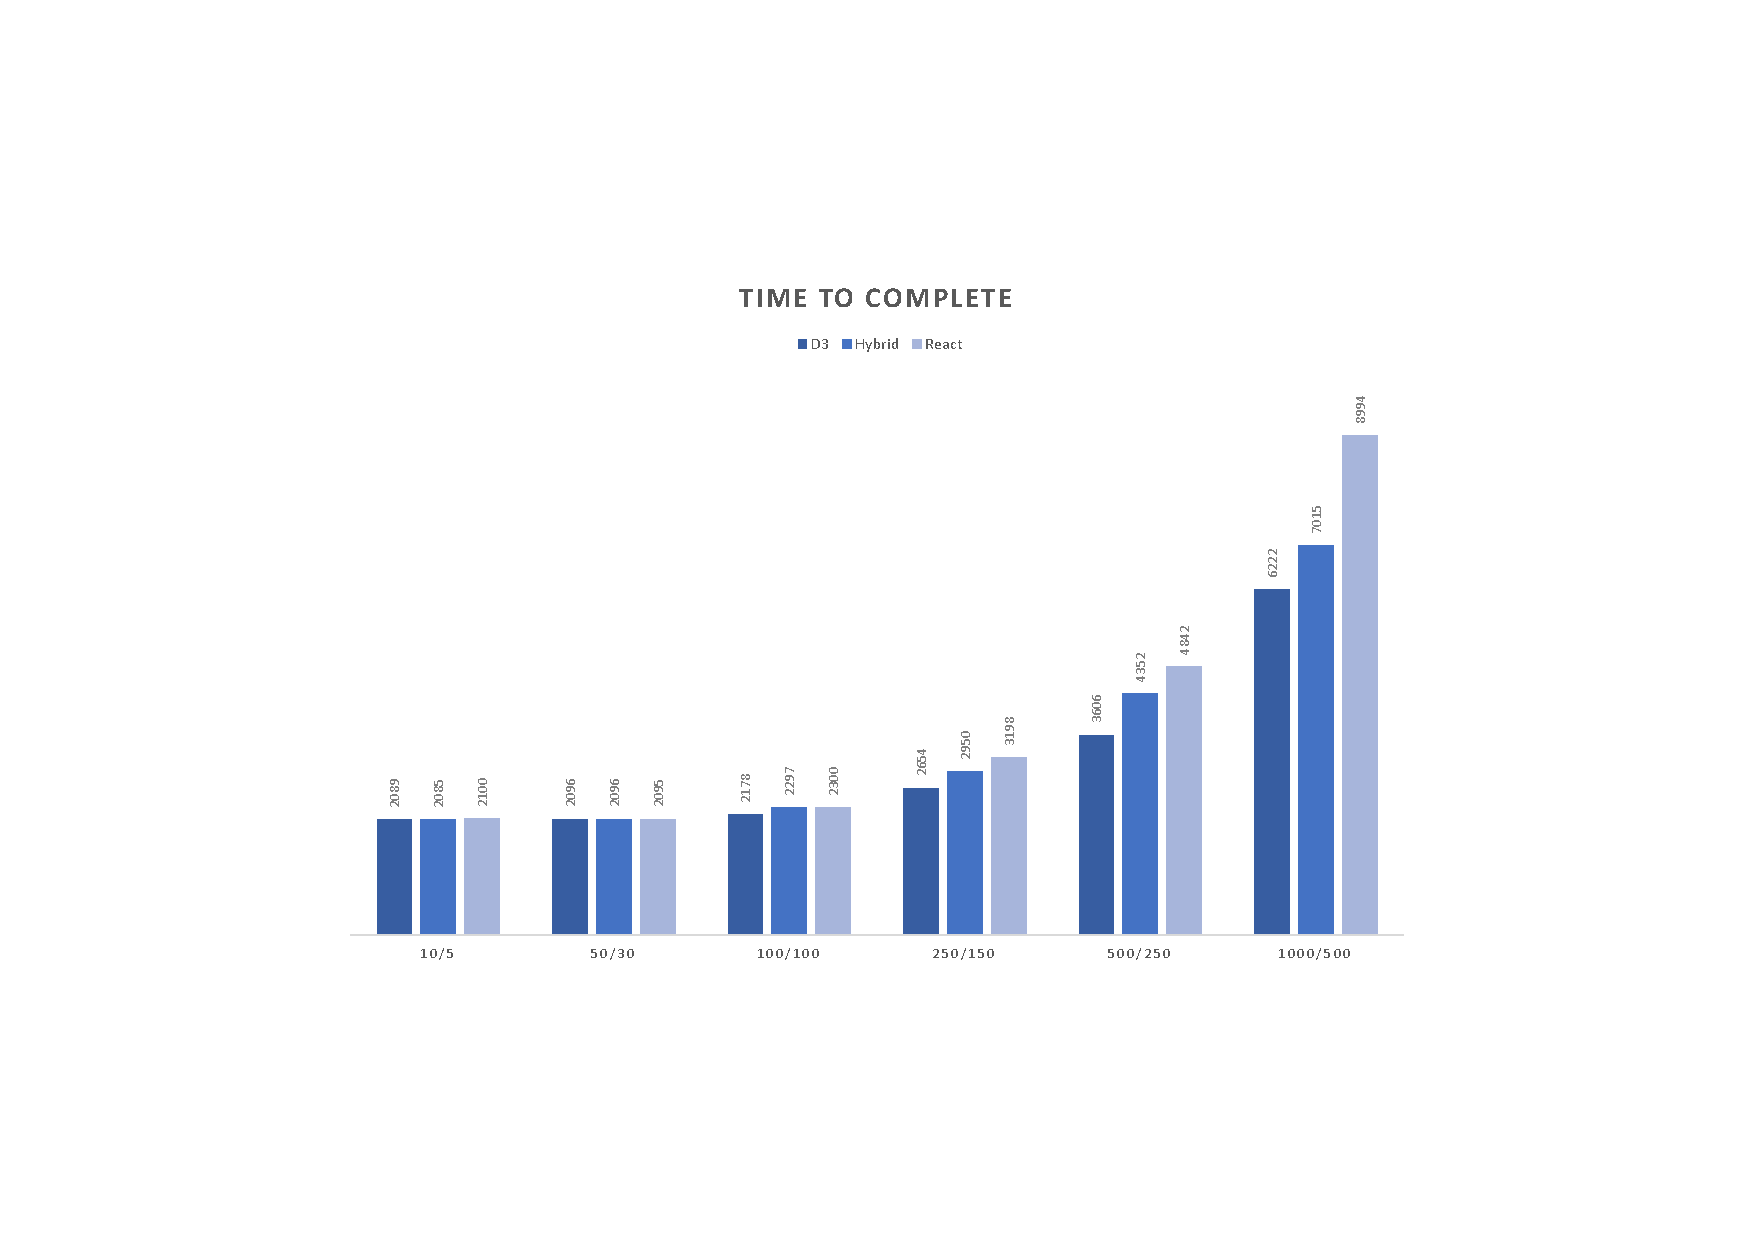
\includegraphics[scale=2.5, trim= 4cm 4cm 4cm 4cm, clip, width=1\columnwidth]{perfHighEnd002.pdf}
\caption{Average time to complete for one benchmark iteration cycle in milliseconds}
\label{fig:perfHighEnd002}
\end{figure}

\begin{figure}
\centering
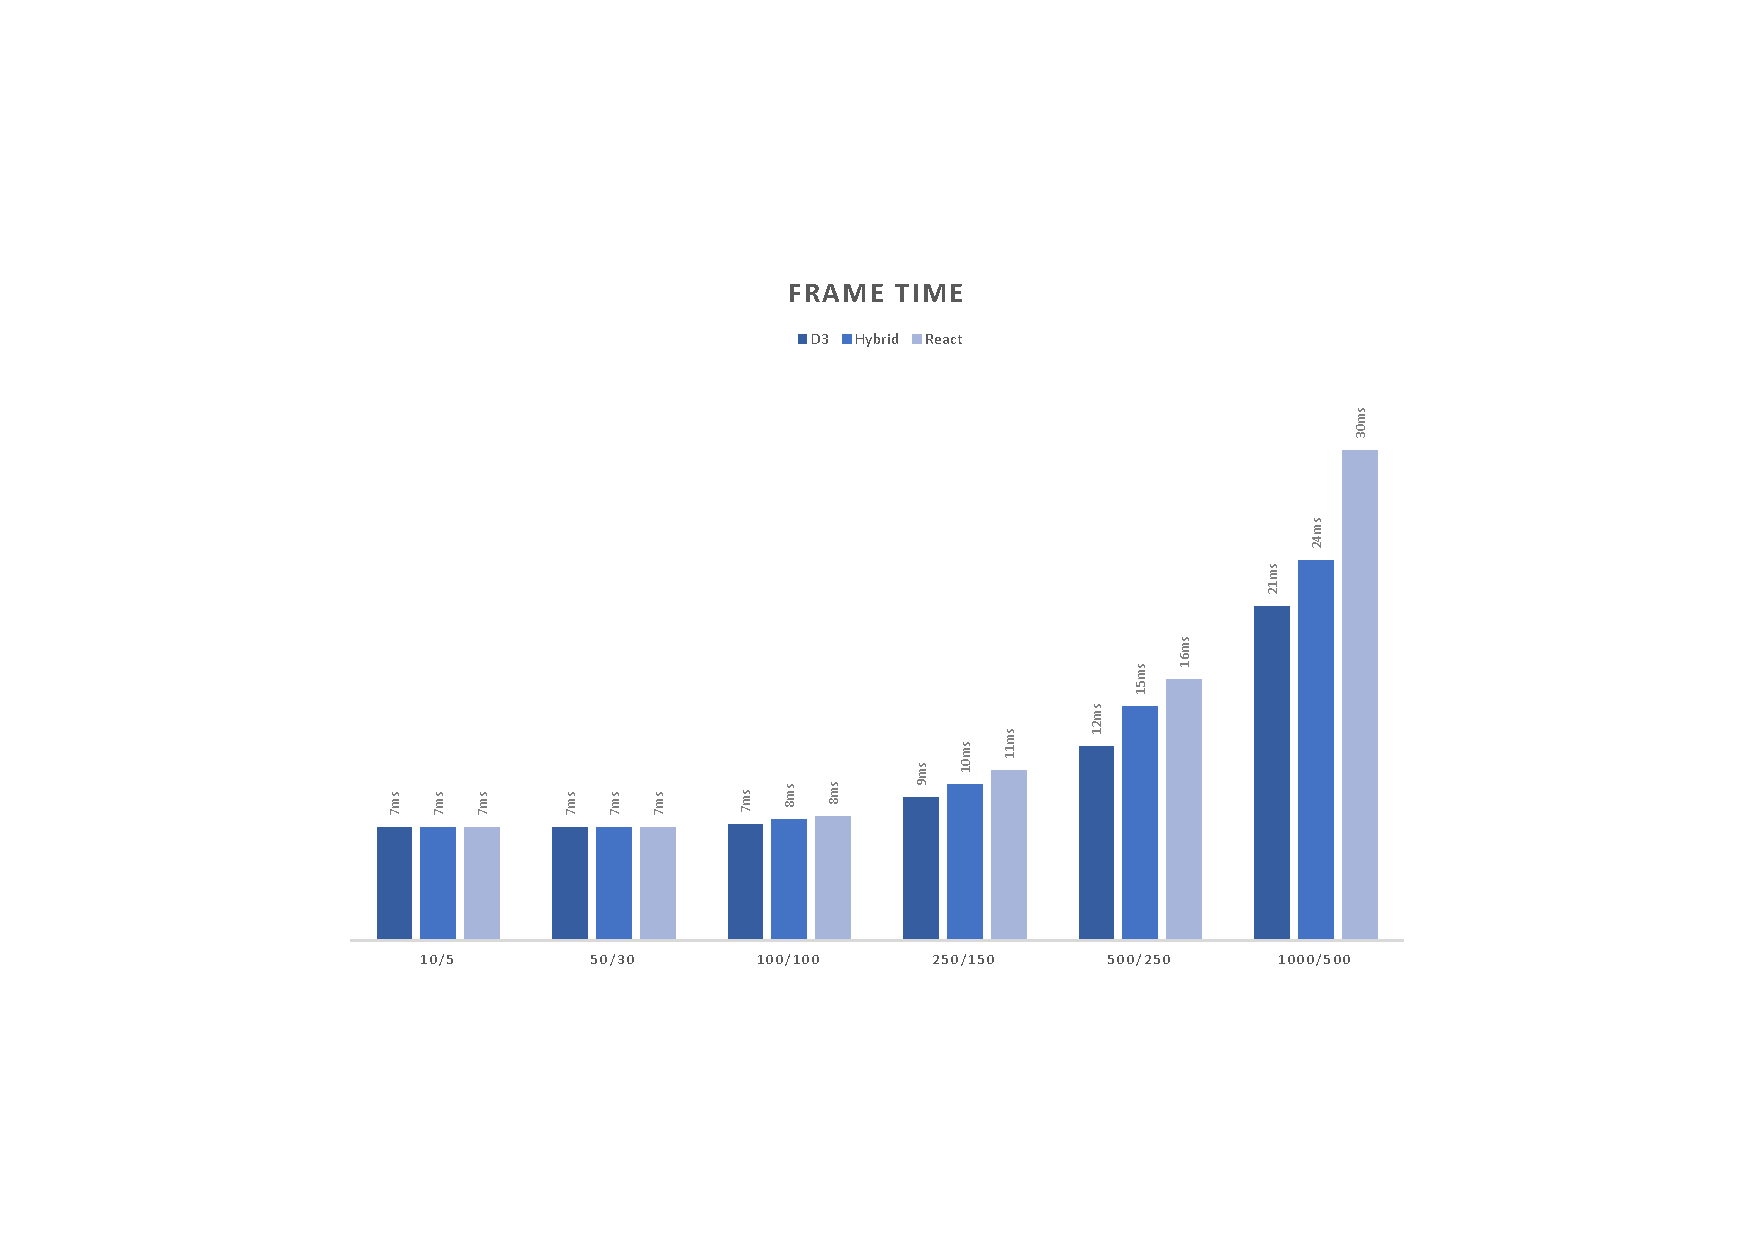
\includegraphics[scale=2.5, trim= 4cm 4cm 4cm 4cm, clip, width=1\columnwidth]{perfHighEnd003.pdf}
\caption{Average frametime per benchmark iteration cycle}
\label{fig:perfHighEnd003}
\end{figure}

\begin{figure}
\centering
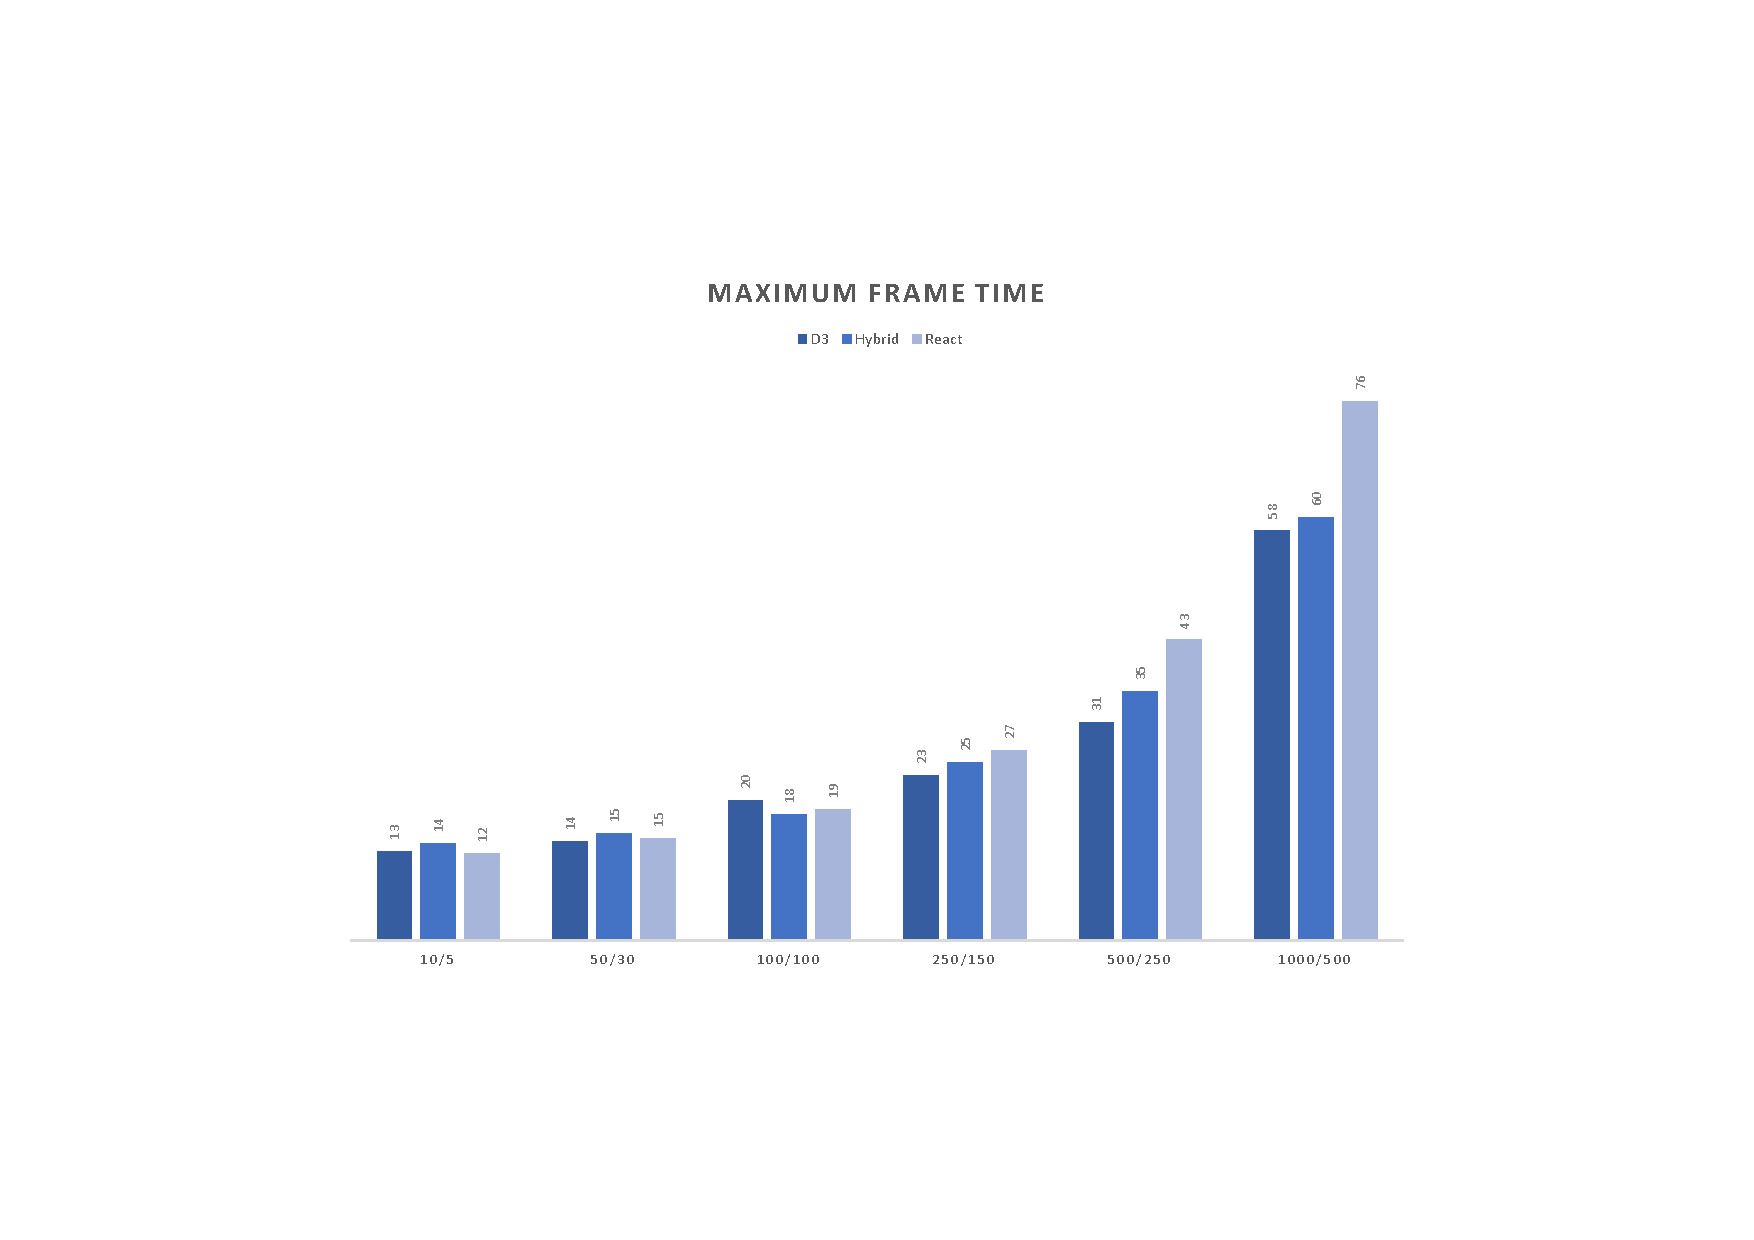
\includegraphics[scale=2.5, trim= 4cm 4cm 4cm 4cm, clip, width=1\columnwidth]{perfHighEnd004.pdf}
\caption{Average maximum frametime per benchmark iteration cycle}
\label{fig:perfHighEnd004}
\end{figure}

\subsection{Human Perception of fluid animations}

\subsection{Interpreting the test results}

\section{Conclusion}

